% !TeX spellcheck = en_GB
% !TeX encoding = UTF-8
% !TeX root = exp_SAE.tex
% !TeX TS-program = pdflatex
% !BIB TS-program = biber

\documentclass[sigconf,natbib=false, language=english]{acmart}

\usepackage[datamodel=acmdatamodel, style=acmnumeric, backend=biber]{biblatex}
\addbibresource{references.bib}

\AtBeginDocument{%
  \providecommand\BibTeX{{%
    Bib\TeX}}}

\setcopyright{rightsretained}
\copyrightyear{2026}
\acmDOI{10.70314/is.2026.sikdd.89}

\acmConference[Information Society 2026]{Information Society 2026: 29th international multiconference}{5--9 October 2026}{Ljubljana, Slovenia}
\acmISBN{}
\settopmatter{printccs=false, printacmref=false}

\geometry{a4paper}

% Packages for tables and figures
\usepackage{booktabs}
\usepackage{float}
\usepackage{subcaption}

\begin{document}

\title[SAE Features for Headline A/B Tests]{Explaining Headline A/B Test Outcomes with Sparse Autoencoder Features}

\author{Drejc Pesjak}
\affiliation{%
  \institution{Jo\v{z}ef Stefan Institute}
  \institution{Jo\v{z}ef Stefan International Postgraduate School}
  \city{Ljubljana}
  \country{Slovenia}
}
\email{drejc.pesjak@ijs.si}
\orcid{0009-0003-0750-8157}

\author{Dunja Mladeni\'{c}}
\affiliation{%
  \institution{Jo\v{z}ef Stefan Institute}
  \institution{Jo\v{z}ef Stefan International Postgraduate School}
  \city{Ljubljana}
  \country{Slovenia}
}

\author{Jan Rupnik}
\affiliation{%
  \institution{Nordoon Inc.}
  \city{Palo Alto}
  \country{California, USA}
}

\renewcommand{\shortauthors}{D. Pesjak et al.}

\begin{abstract}
A/B testing is a standard method for optimizing news headlines, yet it reveals only \emph{which} variant wins, not \emph{why}. We propose representing headline pairs through Sparse Autoencoder (SAE) features extracted from a large language model. For each within-test pair we construct a \emph{context} vector (shared topic) and a \emph{diff} vector (wording differences), apply histogram-based binarization to suppress activation noise, and train gradient-boosted trees followed by RuleFit to extract interpretable feature patterns. On approximately 57,000 pairs from the Upworthy Research Archive, our best model achieves 61.8\% pairwise accuracy and 0.76 AUC. The dominant predictive features are \emph{diff} features with recognizable labels such as ``clickbait-style framing,'' ``curiosity gaps,'' ``emotional intensity,'' and use of the demonstrative ``this.'' We also test a \emph{hierarchy hypothesis}---that topic context gates which diff features matter---but find no stable topic-gated regimes. The results demonstrate that SAE features provide a viable middle ground between opaque dense embeddings and shallow bag-of-words representations for interpretable text analysis.
\end{abstract}

\keywords{large language models, sparse autoencoders, A/B testing, headline optimization, interpretable machine learning, mechanistic interpretability}

\maketitle

%% ====================================================================
\section{Introduction}
%% ====================================================================

% A/B testing is the gold standard for comparing content variants in digital media: show two headlines to random audiences and measure which one gets more clicks. Yet the outcome of such a test is merely a winner and a loser. Practitioners learn \emph{which} headline performed better but not \emph{why}---making it difficult to transfer insights to future headline writing or to build systematic understanding of what drives engagement.
Many decisions in digital media come down to a choice between two variants of the same
content, where small differences in wording translate into large differences in reach.
A/B testing settles such questions empirically: show both variants to random audiences
and measure which one wins. The outcome, however, is merely a winner and a loser. An
explanation of why would be more useful, as it carries over to headlines that were
never tested.

Moving from winner identification to interpretable explanation requires a text representation that a statistical model can learn from. Early approaches---bag-of-words, TF-IDF, n-grams---are interpretable but miss context and meaning. Dense contextual embeddings from Transformer models~\cite{vaswani2017attention} such as BERT~\cite{devlin2019bert} capture rich semantics but are opaque: no single dimension has a human-readable meaning.

Mechanistic interpretability research offers a promising resolution. Sparse Autoencoders (SAEs)~\cite{bricken2023monosemanticity, cunningham2023sparse} trained on LLM activations decompose dense activation vectors into a much larger, sparse set of features---each corresponding to a recognizable concept such as ``shocking scenarios'' or ``use of the word \emph{this}.'' These features can be labeled automatically~\cite{bills2023language}, and the GemmaScope-2 project~\cite{lieberum2024gemma} provides pre-trained SAEs for the Gemma model family with human-readable descriptions hosted on Neuronpedia.

In this work we use SAE features as the representation layer for analyzing A/B-tested news headlines from the Upworthy Research Archive~\cite{matias2021upworthy}. We encode each headline through Gemma-3-4B-IT\footnote{\href{https://huggingface.co/google/gemma-3-4b-it}{google/gemma-3-4b-it on Hugging Face.}}, decompose the activations with a 16,384-width SAE, and construct pairwise \emph{context + diff} vectors that separate shared topic content from wording differences. After binarizing the features to suppress activation noise, we train XGBoost and RuleFit models to identify which SAE features predict the winner and to extract human-readable rules.

We also investigate a hierarchical regime hypothesis: the possibility that the topic or context of an article gates which ``difference'' features matter for clickability, and test this through unsupervised clustering and model-based recursive partitioning.

% The main contributions of this paper are:
% \begin{enumerate}
%     \item An SAE-based feature representation for pairwise headline A/B test analysis, using context+diff decomposition to separate topic from wording effects.
%     \item A histogram-based binarization method that denoises SAE activations and improves both interpretability and predictive performance.
%     \item An investigation of the hierarchy hypothesis---whether article context gates which diff features matter---through clustering and model-based partitioning.
%     \item Extraction of interpretable features and conjunctive rules that describe clickability in human-readable terms.
% \end{enumerate}

%% ====================================================================
\section{Related Work}
%% ====================================================================

\paragraph{Headline A/B testing and engagement.}
The Upworthy Research Archive~\cite{matias2021upworthy} made a large corpus of real headline A/B tests publicly available for research. Gligori\'{c} et al.~\cite{gligoric2023linguistic} analyzed the same archive with logistic regression on hand-crafted linguistic features (word count, sentiment, named entities, syntactic patterns), finding small but significant effects of specific wording choices on click-through rates. Robertson et al.~\cite{robertson2023negativity} used randomized Upworthy trials to show that negatively worded headlines drive higher consumption. Clickbait detection work~\cite{chakraborty2016stop} has identified surface-level engagement cues such as forward references and sensational language. Our approach differs from all of these in using SAE features, which provide richer, model-derived interpretable dimensions rather than manually defined linguistic variables or opaque dense vectors.

\paragraph{Sparse autoencoders and interpretable text representations.}
Sparse autoencoders trained on neural network activations learn overcomplete dictionaries where individual features correspond to human-recognizable concepts~\cite{bricken2023monosemanticity, cunningham2023sparse}. The GemmaScope project~\cite{lieberum2024gemma} provides pre-trained SAEs for the Gemma model family, including JumpReLU variants~\cite{rajamanoharan2024jumping} that use a learnable threshold to enforce sparsity. Feature labels can be generated automatically by having an LLM describe each feature's activation pattern~\cite{bills2023language}. Most directly related to our work, Movva et al.~\cite{movva2025hypothesaes} train SAEs on sentence embeddings and use L1-penalized logistic regression to select predictive features for hypothesis generation. Our work differs in three ways: (i)~we use residual-stream SAEs rather than embedding-space SAEs, (ii)~we introduce a context+diff decomposition for pairwise comparisons, and (iii)~we use tree-based models and RuleFit for conjunctive rule extraction rather than linear feature selection.

\paragraph{Interpretable machine learning.}
RuleFit~\cite{friedman2008rulefit} combines tree-derived conjunction rules with linear terms, producing models that are both predictive and human-readable. XGBoost~\cite{chen2016xgboost} provides strong gradient-boosted baselines with built-in feature importance. Model-based recursive partitioning (MOB)~\cite{zeileis2008mob} tests for parameter instability across subgroups, offering a principled way to discover heterogeneous treatment effects---we use it to test for topic-gated regime structure.

%% ====================================================================
\section{Methods}
%% ====================================================================

\subsection{Dataset}

We use the Upworthy Research Archive~\cite{matias2021upworthy}, which contains A/B test data from the news website Upworthy. Each ``test'' compared 2--5 headline variants for the same article, with real impression and click counts used to calculate click-through rate (CTR). We use the \emph{confirmatory} split, comprising approximately 13,500 unique test IDs.

After preprocessing (HTML tag removal, deduplication, removal of single-headline tests), we sample within-test headline pairs. For each test with $N$ headlines, we draw up to $\min\bigl(\binom{N}{2},\, 10\bigr)$ random pairs, yielding approximately 57,289 pairs with balanced labels. The pair order is randomized, and the binary label is:
\begin{equation}
    y = \mathbf{1}\bigl[\mathrm{CTR}_A > \mathrm{CTR}_B\bigr]
    \label{eq:label}
\end{equation}
where $\mathrm{CTR} = \text{clicks} / \text{impressions}$ for each headline. We split into training (45,657 pairs) and test (11,632 pairs) sets using \texttt{GroupShuffleSplit} by \texttt{test\_id}, ensuring that all pairs from the same test remain in the same split to prevent data leakage.

\subsection{SAE Feature Extraction}

Each headline is wrapped in a Gemma-3 chat template and passed through Gemma-3-4B-IT (Google's 4-billion parameter instruction-tuned model). We extract residual stream activations $\mathbf{h}_t \in \mathbb{R}^{2560}$ at layer~22 for each token position $t$, masking out instruction template tokens so that only headline content tokens remain.

The content-token activations are then encoded through a pre-trained JumpReLU SAE from the GemmaScope-2 project~\cite{lieberum2024gemma}:
\begin{equation}
    \mathbf{z}_t = \mathrm{JumpReLU}_\theta\!\bigl(\mathbf{W}_{\mathrm{enc}}\,\mathbf{h}_t + \mathbf{b}_{\mathrm{enc}}\bigr)
    \label{eq:sae}
\end{equation}
where $\mathbf{W}_{\mathrm{enc}} \in \mathbb{R}^{d_{\mathrm{SAE}} \times d_{\mathrm{model}}}$, $d_{\mathrm{SAE}} = 16{,}384$, and the JumpReLU activation sets entries below a learned threshold $\theta$ to zero:
\begin{equation}
    \mathrm{JumpReLU}_\theta(x) = x \cdot \mathbf{1}[x > \theta]
    \label{eq:jumprelu}
\end{equation}

To obtain a single vector per headline, we max-pool across all content token positions:
\begin{equation}
    \mathbf{v} = \max_{t \in \mathcal{T}_{\mathrm{content}}} \mathbf{z}_t
    \label{eq:maxpool}
\end{equation}
yielding a sparse vector $\mathbf{v} \in \mathbb{R}^{16384}_{\geq 0}$ where each dimension corresponds to a named SAE feature (e.g., ``discovery and revelation,'' ``shocking scenarios'').

\subsection{Pairwise Context + Diff Representation}

Predicting CTR from a single headline's SAE vector would mostly capture which \emph{topics} are inherently popular, not what makes one headline beat another for the same article. Since we have within-test pairs, we can focus on wording differences.

For a pair $(A, B)$ with SAE vectors $\mathbf{v}_A$ and $\mathbf{v}_B$, we compute:
\begin{align}
    \mathbf{c} &= \frac{\mathbf{v}_A + \mathbf{v}_B}{2} & &\text{(context: shared topic/content)} \label{eq:context} \\
    \mathbf{d} &= \mathbf{v}_A - \mathbf{v}_B & &\text{(diff: wording differences)} \label{eq:diff}
\end{align}
and concatenate them into a single feature vector:
\begin{equation}
    \mathbf{x} = [\,\mathbf{c} \;\|\; \mathbf{d}\,] \in \mathbb{R}^{32768}
    \label{eq:concat}
\end{equation}

% The diff vector captures what distinguishes the two headlines---the signal most relevant for predicting the winner. 
The diff vector encodes \emph{wording} (not just word) \emph{differences} between the two variants in the SAE feature basis: it captures whatever changes in the model's representation when the phrasing is altered, from surface cues (e.g., demonstratives, punctuation, syntactic templates) to higher-level semantic or stylistic framing (e.g., emotion, moral framing, curiosity gaps).
The context vector captures the shared topic, included to allow models to potentially learn context-dependent rules (e.g., ``emotional language helps for political articles but not for lifestyle content'').

Each pair is weighted by the absolute CTR difference to emphasize pairs with clearer outcomes:
\begin{equation}
    w = \bigl|\mathrm{CTR}_A - \mathrm{CTR}_B\bigr|
    \label{eq:weight}
\end{equation}

\subsection{Feature Binarization}
\label{sec:binarization}

Raw SAE activations contain noise near the JumpReLU cutoff. The non-zero values exhibit characteristic distributional structure (Figure~\ref{fig:distributions}) that we exploit for denoising.

For \emph{context} features (the per-pair mean activation) the distribution has two overlapping components. When only one headline of the pair fires the feature the mean is half the single-headline activation, producing a steeply decaying exponential just above the JumpReLU cutoff. When both headlines fire, the mean of two draws yields a bell-shaped body at higher values. For \emph{diff} features the distribution has a central Gaussian at zero (both headlines activate the feature similarly), flanked by exponential-like tails shifted into the positive and negative directions (one headline activates the feature substantially more than the other).

We separate noise from signal with a histogram-based ``walk'' threshold. For context, we walk rightward from the smallest non-zero bin: when 4~consecutive bins are all higher than the current bin, the transition from the decaying component to the bell-shaped body has been reached, yielding threshold~$\tau_{c,j}$ and binary encoding $\tilde{c}_j = \mathbf{1}[c_j > \tau_{c,j}]$. For diff features the same walk proceeds outward from zero in both directions, yielding symmetric thresholds $\pm\tau_{d,j}$ and trinary encoding:
\begin{equation}
    \tilde{d}_j = \begin{cases}
        +1 & \text{if } d_j > +\tau_{d,j} \\
        -1 & \text{if } d_j < -\tau_{d,j} \\
        \phantom{+}0 & \text{otherwise}
    \end{cases}
    \label{eq:bin_diff}
\end{equation}

\begin{figure}[h]
    \centering
    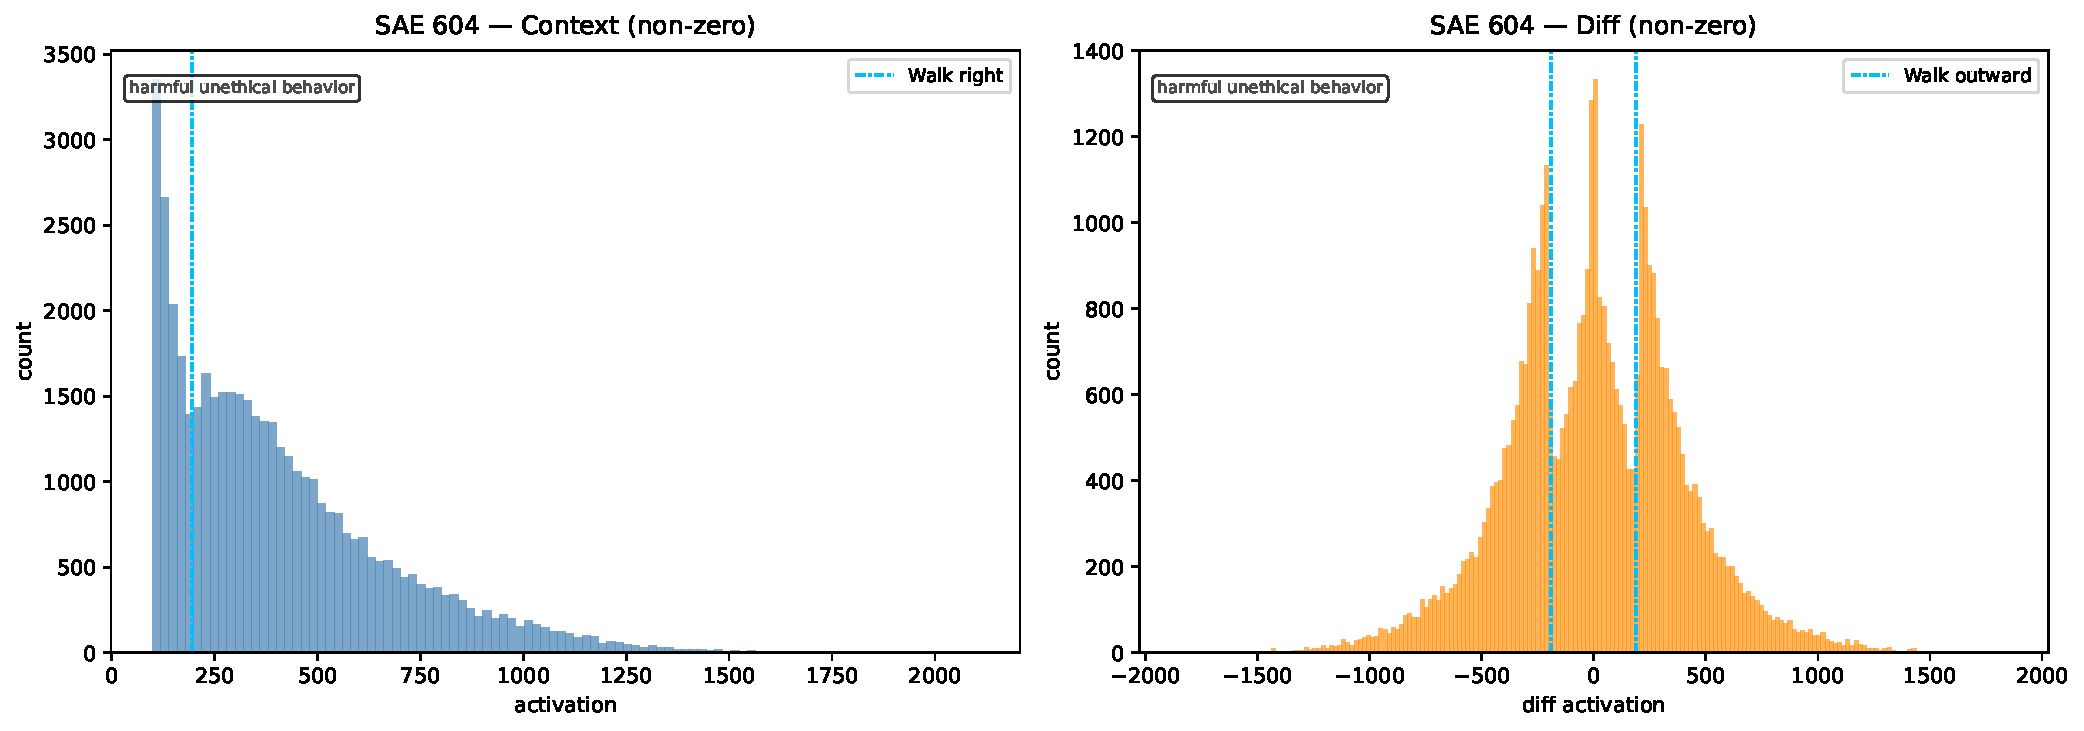
\includegraphics[width=\columnwidth]{figures/feature_604_distributions_walk_threshold.pdf}
    % \caption{Non-zero activation distributions for SAE feature~604 (``harmful unethical behavior''). Left: context (mean) activations show a decaying exponential from single-headline activations overlaid with a bell-shaped body from pairs where both headlines fire; the walk-right threshold (dashed) separates them. Right: diff activations form a central Gaussian at zero flanked by exponential tails; the symmetric walk-outward thresholds (dashed) yield trinary encoding.}
    \caption{Context (left) and difference (right) activations for SAE feature~604 (``harmful unethical behavior''). Dashed lines mark walk thresholds.}
    \Description{Side-by-side histograms of SAE feature 604 mean and diff activations with walk thresholds marked.}
    \label{fig:distributions}
\end{figure}

\subsection{Models}

We evaluate the following models, all on the same group-based train/test split:

\textbf{Logistic Regression.} SGD-trained logistic regression with L2 regularization ($\alpha = 10^{-4}$) on the full 32,768-dimensional continuous feature vectors (we apply StandardScaler without centering to preserve sparsity), serving as a linear baseline.

\textbf{XGBoost on binarized features.} Gradient-boosted trees~\cite{chen2016xgboost} with 100 estimators, maximum depth~6, learning rate~0.1, and column subsampling of~0.7, trained on the binarized/trinarized 32,768 int8 features. Sample weights are set to $w$ (Equation~\ref{eq:weight}). Only 467 out of 32,768 features receive non-zero importance from this model.

\textbf{RuleFit on XGBoost-selected features.} We extract the 467 features with non-zero XGBoost importance and train a RuleFit model~\cite{friedman2008rulefit} (25~estimators, tree size~4, maximum 500~rules). RuleFit generates both linear terms (each binarized feature with a coefficient) and conjunction rules (tree-derived feature combinations), producing a fully interpretable model.

\textbf{Additional baselines.} We also train a depth-8 decision tree (for visual interpretability), XGBoost with depth-1 stumps (to test whether additive features suffice), and per-cluster XGBoost models (to test the hierarchy hypothesis). %Full details are in Table~\ref{tab:results}.

%% ====================================================================
\section{Results}
%% ====================================================================

\subsection{Main Results}

% Table~\ref{tab:results} summarizes all models evaluated on the canonical train/test split with sample weights $w = |\mathrm{CTR}_A - \mathrm{CTR}_B|$.
Experimental evaluation compares all models on the same group-based train/test split
with sample weights $w = |\mathrm{CTR}_A - \mathrm{CTR}_B|$.
Table~\ref{tab:results} summarizes the results giving three commonly used evaluation
metrics: classification accuracy (Acc), harmonic mean of precision and recall (F1) and
area under the Receiver Operating Characteristic curve (AUC).

\begin{table}[ht]
\centering
% \caption{Model comparison on the test set (11,632 pairs). All models use \texttt{GroupShuffleSplit} by \texttt{test\_id}. Best results per metric in \textbf{bold}.}
\caption{Performance of all evaluated models on the held-out test set.}
\label{tab:results}
\begin{tabular}{@{}llccc@{}}
\toprule
\# & Method & Acc & F1 & AUC \\
\midrule
1 & Logistic Regression      & 0.606 & 0.606 & 0.750 \\
2 & Decision Tree            & 0.556 & 0.551 & 0.630 \\
3 & XGBoost (continuous)     & 0.616 & 0.616 & 0.759 \\
4 & XGBoost per-cluster      & 0.571 & 0.564 & 0.673 \\
5 & \textbf{XGBoost (binarized)}      & \textbf{0.618} & \textbf{0.619} & 0.759 \\
6 & XGBoost stumps ($d$=1)   & 0.577 & 0.578 & 0.681 \\
7 & Decision Tree (binarized) & 0.553 & 0.549 & 0.625 \\
8 & RuleFit (467 features)   & 0.588 & 0.556 & \textbf{0.761} \\
\bottomrule
\end{tabular}
\end{table}

% Several patterns emerge from the comparison. Logistic regression is competitive (AUC~0.750), indicating a substantial additive/global signal in the SAE features. XGBoost slightly outperforms LR (AUC~0.759 vs.\ 0.750), suggesting nonlinear feature interactions exist but are not dominant. Depth-6 trees substantially outperform depth-1 stumps (AUC~0.759 vs.\ 0.681), confirming that multi-way feature interactions carry predictive information beyond additive effects. Binarization provides a small but consistent improvement (accuracy 61.6\% $\rightarrow$ 61.8\%), while also concentrating importance on just 467 of 32,768 features. RuleFit achieves comparable AUC (0.761) to the best XGBoost model with a fully interpretable output of 52 conjunction rules and 443 linear terms.
Logistic regression is competitive (AUC~0.750), while XGBoost performs slightly better (0.759), indicating useful but limited nonlinear interactions. Depth-6 trees outperform stumps (0.759 vs.\ 0.681 AUC). Binarization slightly improves accuracy (61.6\% $\rightarrow$ 61.8\%) and concentrates importance on 467 of 32,768 features. RuleFit reaches comparable AUC (0.761) with 52 conjunction rules and 443 linear terms.

\subsection{Top Predictive Features}

Table~\ref{tab:top_features} shows the ten most important linear terms from the RuleFit model. All are \emph{diff} features---the SAE dimensions that capture how two headlines differ---confirming that \emph{what distinguishes the headlines} matters far more than \emph{what the article is about}. Context features appear only rarely among the top importances.

\begin{table}[t]
\centering
\caption{Top 10 RuleFit linear terms by importance. All are diff features. A positive coefficient means that headline~A activating this feature more than headline~B predicts that A wins (higher CTR).}
\label{tab:top_features}
\begin{tabular}{@{}clcc@{}}
\toprule
Rank & SAE Feature Label & Coef & Imp \\
\midrule
1 & ``this'' (demonstrative) & $+$0.14 & 0.076 \\
2 & clickbait-style titles & $+$0.11 & 0.070 \\
3 & remarkable, amazing qualities & $+$0.11 & 0.068 \\
4 & discovery and revelation & $+$0.10 & 0.061 \\
5 & subtitles & $-$0.12 & 0.061 \\
6 & past actions or events & $+$0.11 & 0.059 \\
7 & shocking or horrifying scenarios & $+$0.10 & 0.057 \\
8 & harmful unethical behavior & $+$0.08 & 0.056 \\
9 & math and trick questions & $+$0.09 & 0.056 \\
10 & stereotypes about gender roles & $+$0.09 & 0.055 \\
\bottomrule
\end{tabular}
\end{table}

The features tell a coherent story: headlines that use the demonstrative ``this'' (creating a curiosity gap), employ clickbait-style framing, evoke emotional intensity (shock, outrage), or promise revelation tend to get more clicks. Dry, subtitle-style text (feature~5, negative coefficient) hurts clickability.

\subsection{Example Interpretable Rules}

% Beyond linear terms, RuleFit produces conjunction rules that capture feature interactions. Table~\ref{tab:rules} shows selected examples. These rules combine multiple binarized SAE features, illustrating how clickability depends on feature combinations rather than any single dimension.
Table~\ref{tab:rules} shows selected RuleFit conjunction rules capturing interactions among binarized SAE features.

\begin{table}[t]
\centering
% \caption{Selected RuleFit conjunction rules. ``$> 0.5$'' on a binarized diff feature means headline~A activates it more; ``$\leq -0.5$'' means B activates it more.}
\caption{Examples of interpretable conjunction rules extracted by RuleFit. Positive and negative diff values favor headline A and B, respectively.}
\label{tab:rules}
\small
\begin{tabular}{@{}c p{0.8\columnwidth} c@{}}
\toprule
\# & Rule & Coef \\
\midrule
1 & \texttt{clickbait titles} $> 0.5$ & $+$0.07 \\
2 & \texttt{unexpected things} $> 0.5$ & $+$0.06 \\
3 & \texttt{intense negative emotions} $\leq -0.5$ & $-$0.05 \\
4 & \texttt{recognizing or noticing} $\leq -0.5$ & $-$0.14 \\
5 & \texttt{joke, humor} $> {-}0.5$ and \texttt{things or anything} $\leq 0.5$ and ctx: \texttt{asking questions} $> 0.5$ & $+$0.03 \\
6 & \texttt{regulation, risk} $> 0.5$ and \texttt{past events} $> {-}0.5$ & $-$0.04 \\
\bottomrule
\end{tabular}
\end{table}

For instance, the fifth rule states that in the context of question-framed articles (context feature active), if the diff in humor is not strongly negative and the diff in ``things or anything'' vagueness is low, the more humorous variant tends to win. The sixth rule shows that regulatory/governance language combined with past-event framing \emph{hurts} clickability.

\paragraph{Illustrative headline pair.}
Consider a real A/B test from the Upworthy archive where variant~A is \emph{``The Secret About Work Life In 20 Other Countries That Will Surprise You''} and variant~B is \emph{``In Japan, They Have A Word For Working Yourself To Death.''}
Both headlines cover the same topic (international work culture), so their context vectors are similar. However, variant~A strongly activates the diff features for ``clickbait-style titles'' ($+1$) and ``discovery and revelation'' ($+1$) through its ``The Secret\ldots That Will Surprise You'' framing, while variant~B is specific and informative but does not trigger these engagement features. The model predicts~A as the winner, consistent with the observed A/B test outcome.

\subsection{Hierarchy Hypothesis}

A central question was whether \emph{context-dependent rules} govern clickability---for example, whether emotional language helps for political headlines but hurts for lifestyle content. We tested this through three approaches:

\textbf{K-Means clustering} on SVD-reduced context vectors (10~clusters) followed by per-cluster XGBoost models. The aggregated per-cluster predictions achieved 57.1\% accuracy (vs.\ 61.8\% global), a 4.7 percentage point degradation. The clusters fragmented the data without capturing distinct clickability regimes.

\textbf{Model-Based Recursive Partitioning (MOB)}~\cite{zeileis2008mob} using context features as splitting variables and per-leaf Lasso regression on diff features. The MOB tree found statistically significant parameter instability (via the supLM test), producing 10~leaves with different regression coefficients. However, performance was severely overfit: train~$R^2 = 0.39$ vs.\ test~$R^2 = 0.04$, because each leaf had too few samples relative to the 16,384 diff features.

\textbf{XGBoost tree dump analysis.} We audited the split variables in the depth-6 binarized XGBoost model. Of 1,553 total splits, only 188 were on context features (12.1\%), with the remaining 1,365 on diff features. Context splits appeared primarily near leaves, not at the root---suggesting the ensemble does not implement ``context-first gating'' in any strong sense.

These results indicate that while non-additive interactions exist (depth-6 substantially outperforms depth-1 stumps), they are predominantly \emph{among diff features}---not between context and diff. The hierarchy hypothesis, as tested, is not supported.

% %% ====================================================================
% \section{Discussion}
% %% ====================================================================
% Our experimental analysis has shown that on our data
% the best model achieves 61.8\% accuracy and 0.76 AUC---a modest but real signal given that many A/B test pairs have very small CTR differences, making the ground-truth label itself noisy. The SAE features come from a general-purpose LLM not fine-tuned for headline effectiveness, yet they capture recognizable engagement patterns. Across all models, diff features dominate: \emph{what distinguishes two headlines} matters far more than \emph{what the article is about}. The top features---clickbait framing, curiosity gaps, emotional intensity, use of ``this''---align with known headline optimization principles, providing independent empirical validation. Depth-6 trees outperform depth-1 stumps by 7.8 AUC points, confirming that multi-way feature interactions carry signal, yet our attempts to find stable \emph{topic-gated} regimes were unsuccessful---the interactions are among diff features themselves rather than context-diff gating.

% \paragraph{Limitations.}
% The multi-stage pipeline compounds approximation errors, and SAE feature labels---generated automatically---may not perfectly describe what each feature detects. All reported associations are predictive, not causal: without controlled experiments we cannot claim that activating a particular SAE feature \emph{causes} more clicks. Hard partitioning methods (k-means, MOB) may also miss soft or overlapping regime structure.

% %% ====================================================================
% \section{Conclusion}
% %% ====================================================================

% We demonstrated that Sparse Autoencoder features extracted from a large language model provide an interpretable representation for analyzing headline A/B test outcomes. The context + diff decomposition, combined with histogram-based binarization, yields a pipeline that achieves modest but real predictive performance (AUC~0.76) while producing human-readable feature importances and conjunctive rules. The dominant predictive patterns---clickbait framing, curiosity gaps, emotional language, and demonstrative pronouns---align with known engagement heuristics, validating SAE features as a middle ground between opaque embeddings and shallow bag-of-words representations.

% Our investigation of topic-gated hierarchical structure produced informative negative results: while feature interactions exist, stable topic-dependent regimes did not emerge. Future work could explore larger SAE dictionaries (65k or 262k width), models fine-tuned for headline tasks, causal validation through controlled generation, and soft mixture-of-experts approaches to regime discovery.


%% ====================================================================
\section{Discussion and Conclusions}
%% ====================================================================
Our experimental analysis has shown that on our data the best model achieves 61.8\%
accuracy and 0.76 AUC. This is a modest but real signal, given that many A/B test pairs
have very small CTR differences, which makes the ground-truth label itself noisy. The
SAE features come from a general-purpose LLM that was never fine-tuned for headline
effectiveness, yet they capture recognizable engagement patterns. Across all models the
diff features dominate, so what distinguishes two headlines matters far more than what
the article is about. The top features (clickbait framing, curiosity gaps, emotional
intensity, use of ``this'') align with known headline optimization principles and
provide independent empirical validation. Depth-6 trees outperform depth-1 stumps by
7.8 AUC points, suggesting that multi-way feature interactions carry signal, yet our
attempts to find stable topic-gated regimes were unsuccessful. The interactions are
among the diff features themselves rather than between context and diff, an informative
negative result suggesting that hierarchical structure, if present, does not follow the
topic dimension we assumed.

We conclude that Sparse Autoencoder features extracted from a large language model
provide an interpretable representation for analyzing headline A/B test outcomes. The
context + diff decomposition, combined with histogram-based binarization, produces
human-readable feature importances and conjunctive rules at predictive performance
comparable to continuous representations, placing SAE features between opaque dense
embeddings and shallow bag-of-words representations.

\paragraph{Limitations and future work.}
The multi-stage pipeline compounds approximation errors, and the SAE feature labels are
generated automatically, so they may not perfectly describe what each feature detects.
All reported associations are predictive rather than causal: without controlled
experiments we cannot claim that activating a particular SAE feature causes more
clicks. Hard partitioning methods (k-means, MOB) may also miss soft or overlapping
regime structure. Future work could explore larger SAE dictionaries (65k or 262k
width), models fine-tuned for headline tasks, causal validation through controlled
generation, and soft mixture-of-experts approaches to regime discovery.
Future work should compare SAE features against lexical and dense representations
and isolate the contributions of context and binarization through controlled ablations.

%% ====================================================================
\begin{acks}
This research was financially supported by the Slovenian Research and Innovation Agency (ARIS)
through the Young Researcher Grant (PR-13856), the research program Knowledge
Technologies (P2-0103) and the Gravity project AI for Science (GC-0001) and European HE
project DataPact (GA 101189771).

The authors acknowledge the use of Claude to support paper organization
and language and grammar refinement. All AI-generated suggestions were carefully
reviewed and revised by the authors, who take full responsibility for the content
of this paper.
\end{acks}

\printbibliography

\end{document}
